%(BEGIN_QUESTION)
% Copyright 2006, Tony R. Kuphaldt, released under the Creative Commons Attribution License (v 1.0)
% This means you may do almost anything with this work of mine, so long as you give me proper credit

Bestem hva som skjer i følgende trinn i sekvensen (der du blir bedt om svar) i dette kalibreringsoppsettet for trykktransmitter:

$$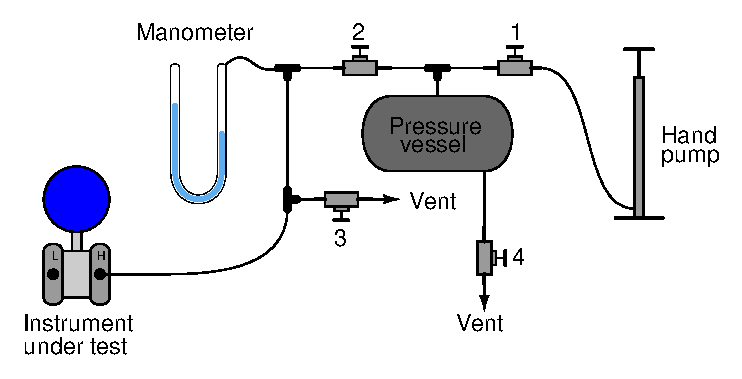
\includegraphics[width=15.5cm]{i00463x01.eps}$$

\begin{itemize}
\item{} {\bf Trinn 1:} Åpne ventiler 1 og 2
\vskip 5pt
\item{} {\bf Trinn 2:} Lukk ventiler 3 og 4
\vskip 5pt
\item{} {\bf Trinn 3:} Betjen håndpumpen til manometeret viser maksimalt trykk
\vskip 5pt
\item{} {\bf Trinn 4: (4 poeng)} Åpne og lukk ventil 4 raskt -- {\it faller manometerindikasjonen mye, litt eller ikke i det hele tatt?}
\vskip 5pt
\item{} {\bf Trinn 5:} Lukk ventil 2
\vskip 5pt
\item{} {\bf Trinn 6: (4 poeng)} Åpne og lukk ventil 4 raskt -- {\it faller manometerindikasjonen mye, litt eller ikke i det hele tatt?}
\vskip 5pt
\item{} {\bf Trinn 7:} Lukk ventil 1
\vskip 5pt
\item{} {\bf Trinn 8: (4 poeng)} Åpne og lukk ventil 3 raskt -- {\it faller manometerindikasjonen mye, litt eller ikke i det hele tatt?}
\end{itemize}

\underbar{file i00463}
%(END_QUESTION)





%(BEGIN_ANSWER)

\begin{itemize}
\item{} {\bf Trinn 4:} Åpne og lukk ventil 4 raskt -- manometeret faller {\bf litt}
\item{} {\bf Trinn 6:} Åpne og lukk ventil 4 raskt -- manometeret {\bf faller ikke} i det hele tatt
\item{} {\bf Trinn 8:} Åpne og lukk ventil 3 raskt -- manometeret faller {\bf mye}
\end{itemize}

%(END_ANSWER)





%(BEGIN_NOTES)

\vskip 20pt \vbox{\hrule \hbox{\strut \vrule{} {\bf Virtuell feilsøking} \vrule} \hrule}

Denne oppgaven egner seg godt som en «virtuell feilsøkingsøvelse». Når du viser diagrammet til elevene, tenker du først ut en bestemt feil i systemet. Deretter presenterer du ett eller flere symptomer på feilen (noe en operatør eller annen bruker kan observere). Elevene foreslår så ulike diagnostiske tester for å finne feiltype og feilsted, som om de var teknikere i virkelig feilsøking. Din oppgave er å oppgi hvilket resultat hver foreslåtte test ville gitt, og dokumentere resultatene slik at alle elevene ser dem.

Under og etter øvelsen er det nyttig å stille oppfølgingsspørsmål som:

\begin{itemize}
\item{} Hva forteller resultatet av den siste diagnostiske testen om feilen?
\item{} Anta at resultatet av den siste testen var annerledes. Hva ville det da fortelle om feilen?
\item{} Er den siste diagnostiske testen den beste vi kunne gjort?
\item{} Hva ville vært ideell rekkefølge på testene for å diagnostisere problemet i færrest mulig trinn?
\end{itemize}

%INDEX% Measurement, pressure: manometer

%(END_NOTES)
